\documentclass[lettersize,journal]{IEEEtran}
\usepackage{amsmath,amsfonts}
\usepackage{algorithmic}
\usepackage{algorithm}
\usepackage{array}
\usepackage[caption=false,font=normalsize,labelfont=sf,textfont=sf]{subfig}
\usepackage{textcomp}
\usepackage{stfloats}
\usepackage{url}
\usepackage{verbatim}
\usepackage{graphicx}
\usepackage{cite}
\hyphenation{op-tical net-works semi-conduc-tor IEEE-Xplore}
% updated with editorial comments 8/9/2021

\begin{document}

\title{Design of a Programmable Multi-Channel Neural Stimulator with SPI-Based Control}

\author{Yiling Xie\\ Department of Electrical and Computer Engineering\\
Rice University, Houston, Texas, USA\\
Email: yx108@rice.edu}
        % <-this % stops a space
\maketitle

\begin{abstract}

This work presents a compact multi-channel neural stimulation system with programmable stimulation control. The proposed architecture includes a high-voltage biphasic stimulator, an SPI-based programmable control system, and a multi-domain power supply structure. To reduce the area overhead associated with high-voltage switching circuits, a current-source-based stimulator architecture is adopted, where switching is performed in the low-voltage domain by controlling the bias currents of current sources. This approach minimizes the number of high-voltage devices while maintaining sufficient voltage compliance for neural stimulation. Stimulation parameters, including pulse timing, polarity, and amplitude, are digitally configured through an SPI interface and a counter-based timing control circuit. The system is implemented in a 180\,nm BCD process. A single stimulator cell occupies $358\,\mu m \times 96\,\mu m$, and the SPI configuration block programs four channels using a 132-bit control word. Simulation results demonstrate programmable biphasic stimulation with a maximum current of 22.5\,µA.

\end{abstract}

\begin{IEEEkeywords}
Stimulator, SPI, power management, wireless power transfer.
\end{IEEEkeywords}

\section{Introduction}
\IEEEPARstart{M}{any} neurological disorders are associated with abnormal neural activity patterns, such as Parkinson’s disease, epilepsy, and chronic pain. Neural stimulators generate controlled current pulses that are injected into neural tissue through electrodes, making them a key component in neuromodulation systems. In addition to clinical therapy, electrical stimulation is also widely used in neuroscience research and brain–computer interface (BCI) systems for neural modulation and sensory feedback \cite{ref1,ref2,ref3}.

In implantable neural interface systems, the stimulator must generate charge-balanced biphasic current pulses to prevent tissue damage caused by charge accumulation. Sufficient voltage compliance is also required to drive electrodes with varying load impedances \cite{ref4,ref14}. These requirements make the design of high-voltage, programmable, and reliable neural stimulation circuits a key challenge in neural interface IC design.

This work investigates the circuit architecture of a multi-channel neural stimulation system. The system includes three main components. First, a high-voltage biphasic stimulator is designed to generate programmable stimulation currents with sufficient voltage compliance. Second, an SPI-based programmable control system configures stimulation parameters and distributes control signals across channels. Third, a system-level power architecture is developed, where the digital control circuits are powered by an on-chip 1.6~V LDO and the stimulator is powered by external $\pm10$~V supplies. In addition, preliminary exploration of wireless power transfer components, including rectifier circuits and coil structures, is conducted for future wireless-powered systems.

\begin{figure}[!t]
\centering
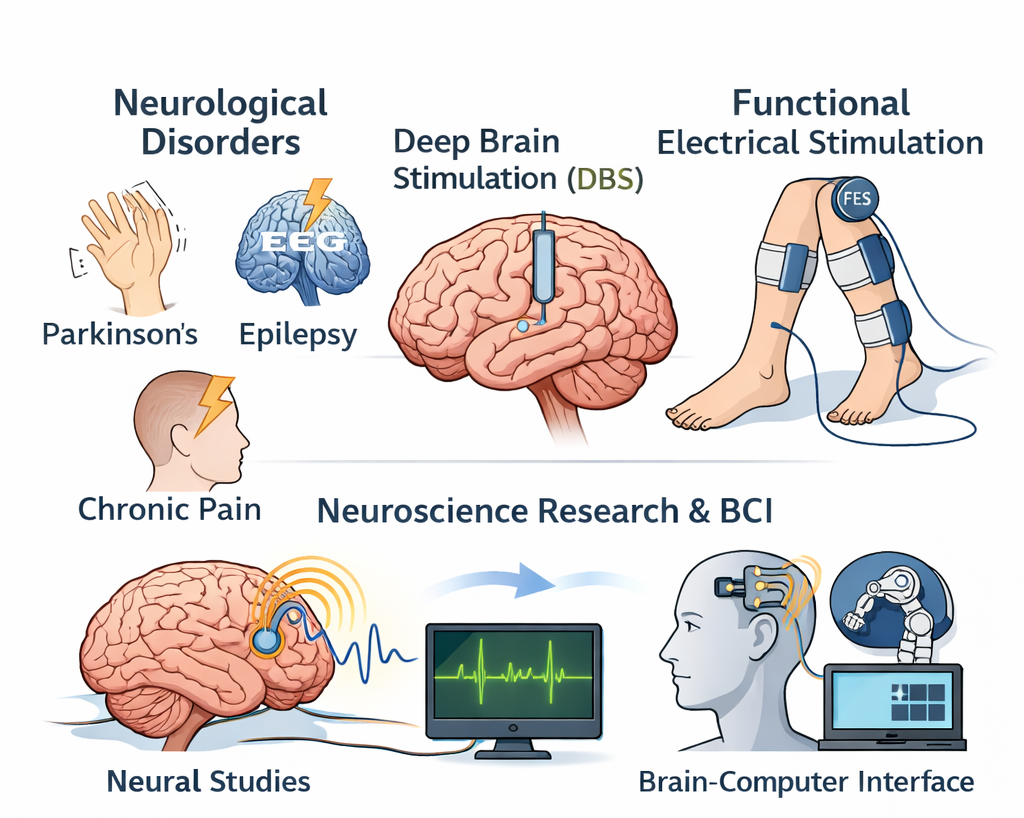
\includegraphics[width=3in]{1}
\caption{Neural Stimulation: Technologies and Applications}
\label{fig_1}
\end{figure}

\section{Methods}
\subsection{High-Voltage Bipolar Stimulator}
In implantable neural interface systems, the stimulator must provide sufficient voltage compliance to accommodate the large impedance variation of the electrode–tissue interface.In a conventional neural stimulator architecture, the stimulation path includes several key circuit blocks. A current-steering DAC generates programmable stimulation current levels, while a local logic control unit produces the timing signals that define the stimulation phases. These low-voltage logic signals are translated through a driver stage to generate the gate-drive voltages required to control the high-voltage stimulation switches connected to the electrode. The driver stage typically consists of level shifters and gate drivers. A discharge-phase circuit is also included to remove residual charge from the electrode–tissue interface and ensure safe biphasic stimulation.

 However, implementing such high-voltage stimulation circuits introduces several design challenges. First, high-voltage (HV) devices occupy significantly larger area than low-voltage devices, limiting the achievable channel density in multi-channel stimulators. Second, as the stimulation voltage increases, the driver circuits must tolerate a larger voltage swing, requiring HV level shifters and additional gate-drive circuitry to generate appropriate intermediate gate voltages for the stimulation switches. These circuits rely on HV devices and introduce significant area overhead, which is critical since area is a primary constraint in this system.

To meet the area limitation, this work adopts a current-source-based stimulator architecture instead of a conventional switched-based stimulator. Fig. 2 illustrates the architecture of the proposed stimulator cell. The stimulation parameters are configured through the SPI interface and stored in the local signal control unit(to be introduced in Section B), which generates the timing signals that define the stimulation phases. A 4-bit current DAC is used to set the stimulation amplitude by selecting different current levels. The generated current is then delivered to the electrode through a current-source-based output stage consisting of programmable source and sink current paths. During the stimulation phase, either the source or sink branch is activated to inject biphasic currents into the neural tissue. The source branch provides positive stimulation current while the sink branch generates the negative phase. To ensure safe neural stimulation, a charge balance circuit is included in the output stage to remove residual charge accumulated at the electrode–tissue interface and maintain charge-balanced operation. By performing the switching and control primarily in the low-voltage domain, the proposed architecture minimizes the number of HV devices. Specifically, the stimulation is controlled by switching the bias currents of the current sources in the low-voltage domain, thereby avoiding HV switching operations.
\begin{figure}[!t]
\centering
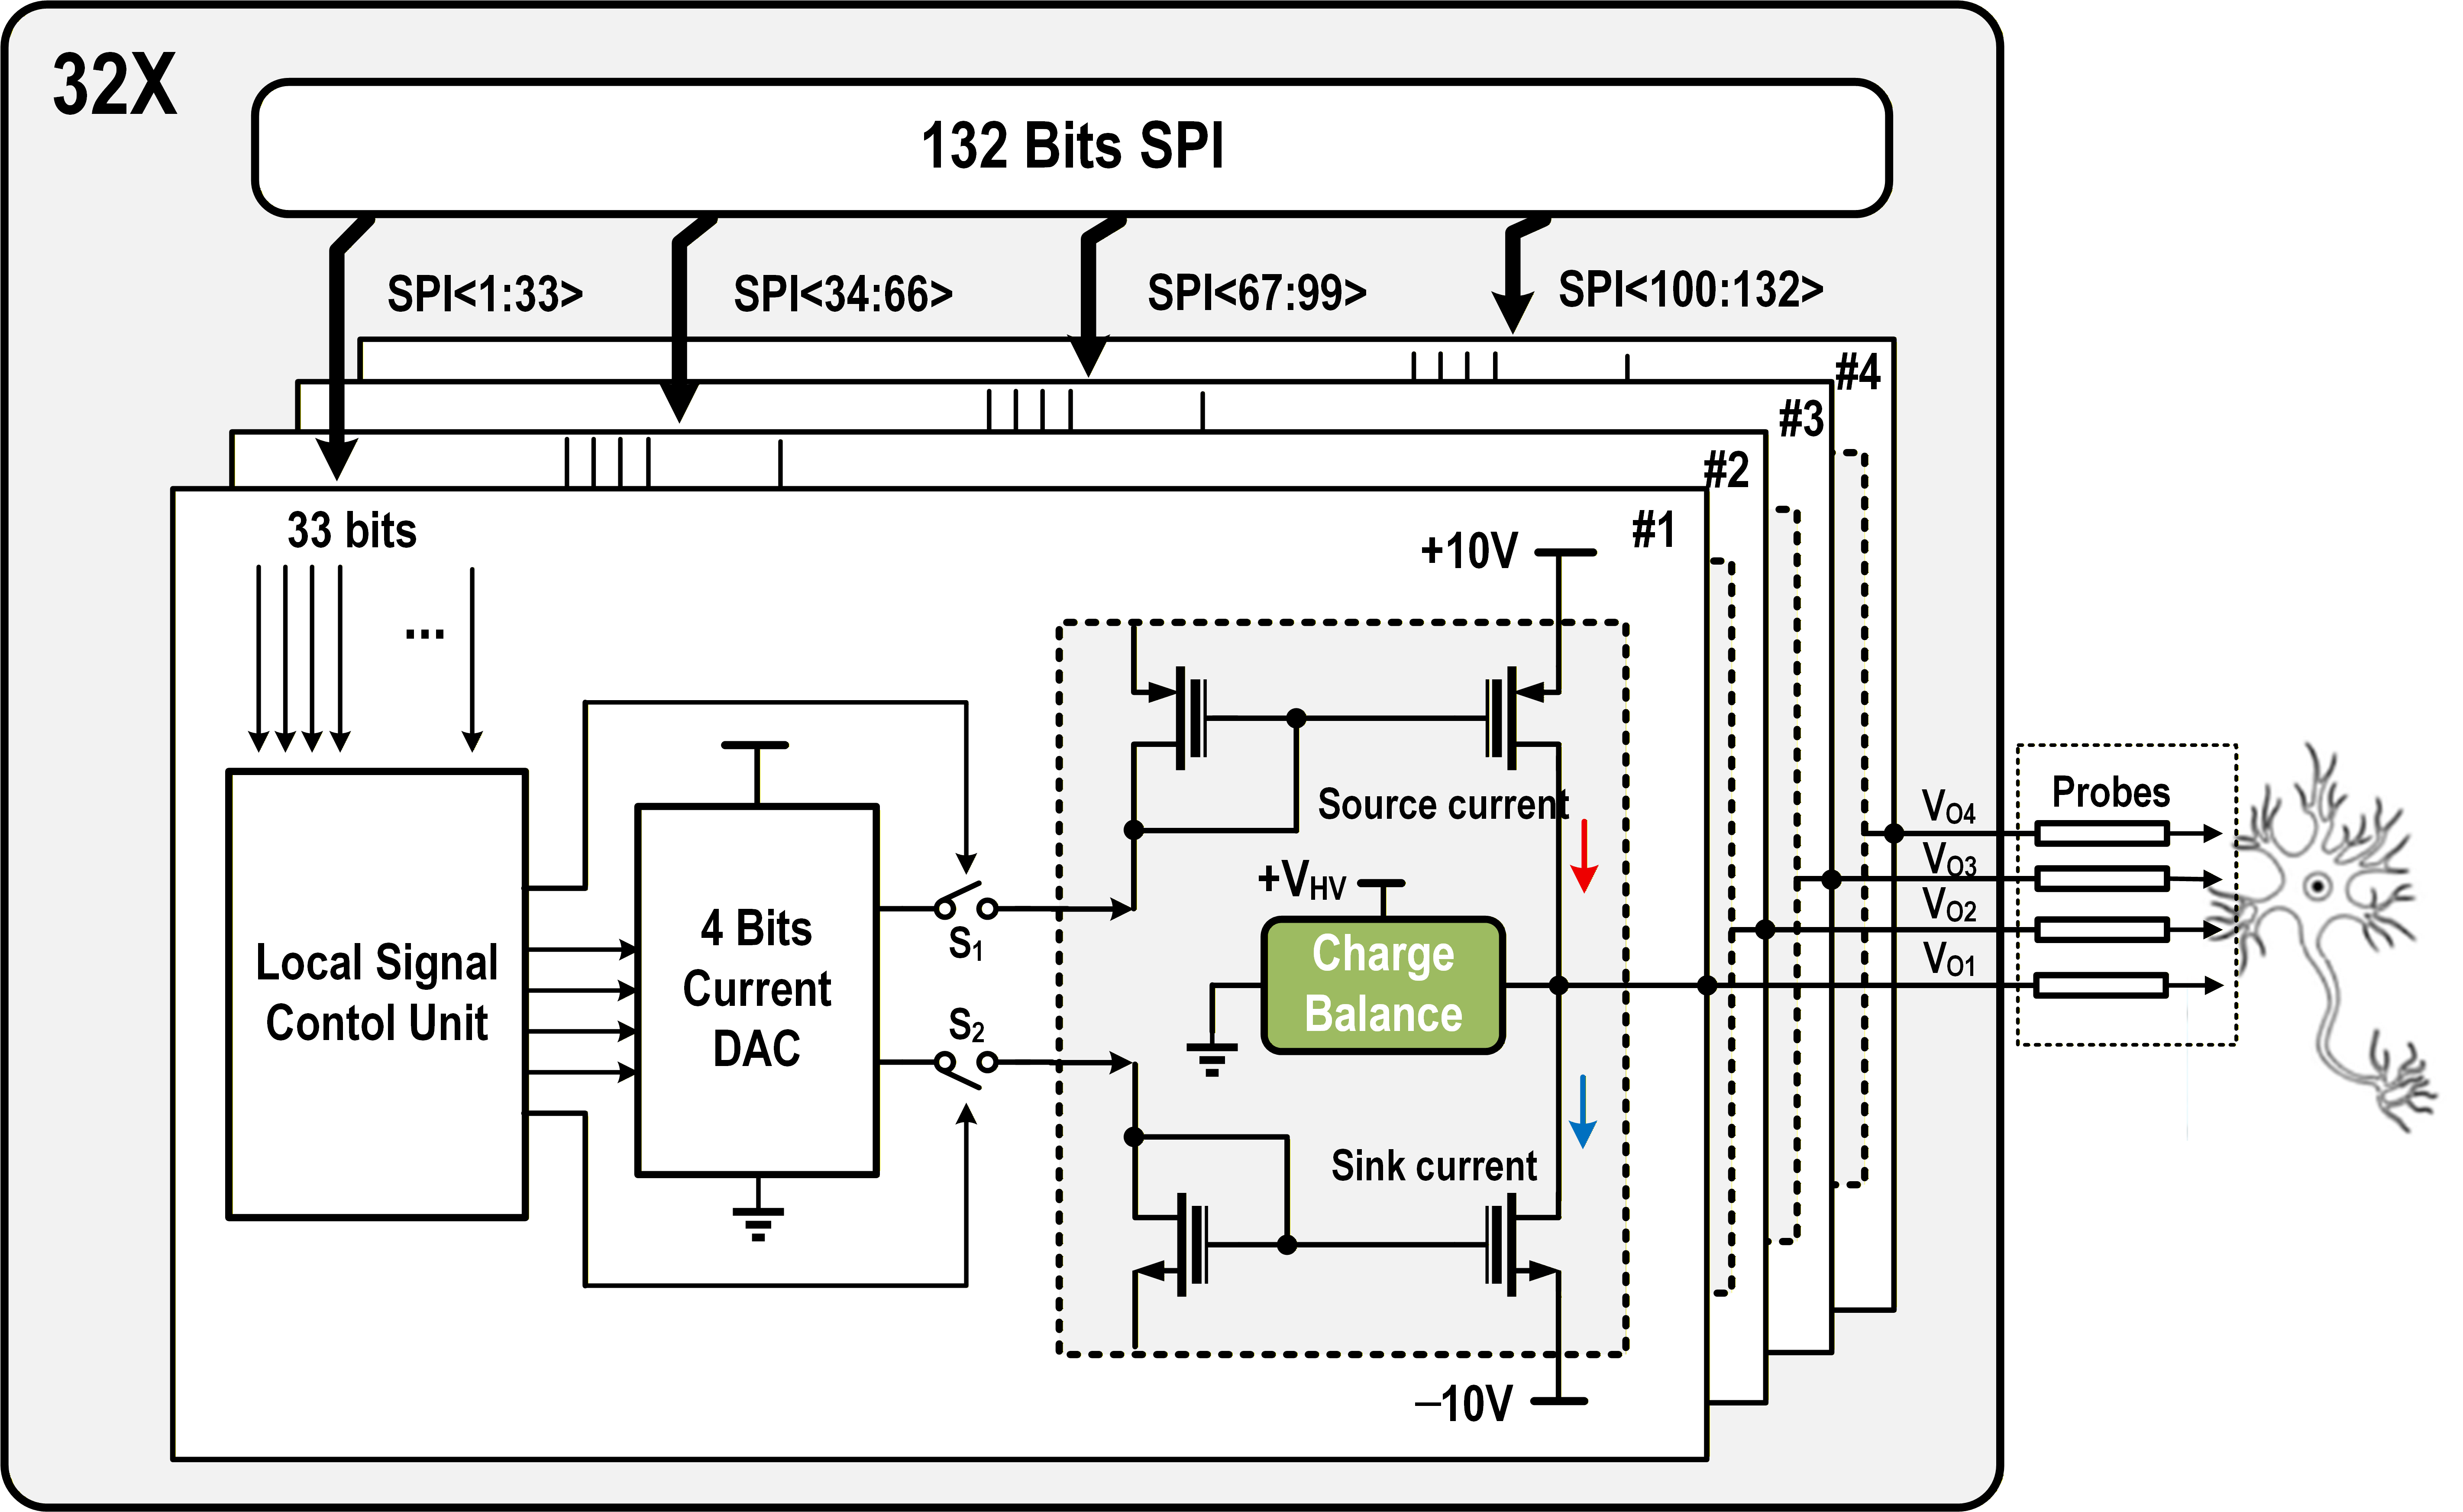
\includegraphics[width=3.5in]{2}
\caption{Neural Stimulation: Technologies and Applications}
\label{fig_2}
\end{figure}

\subsection{SPI-Based Programmable Control for Multi-Channel Stimulation}

\begin{figure}[!t]
\centering
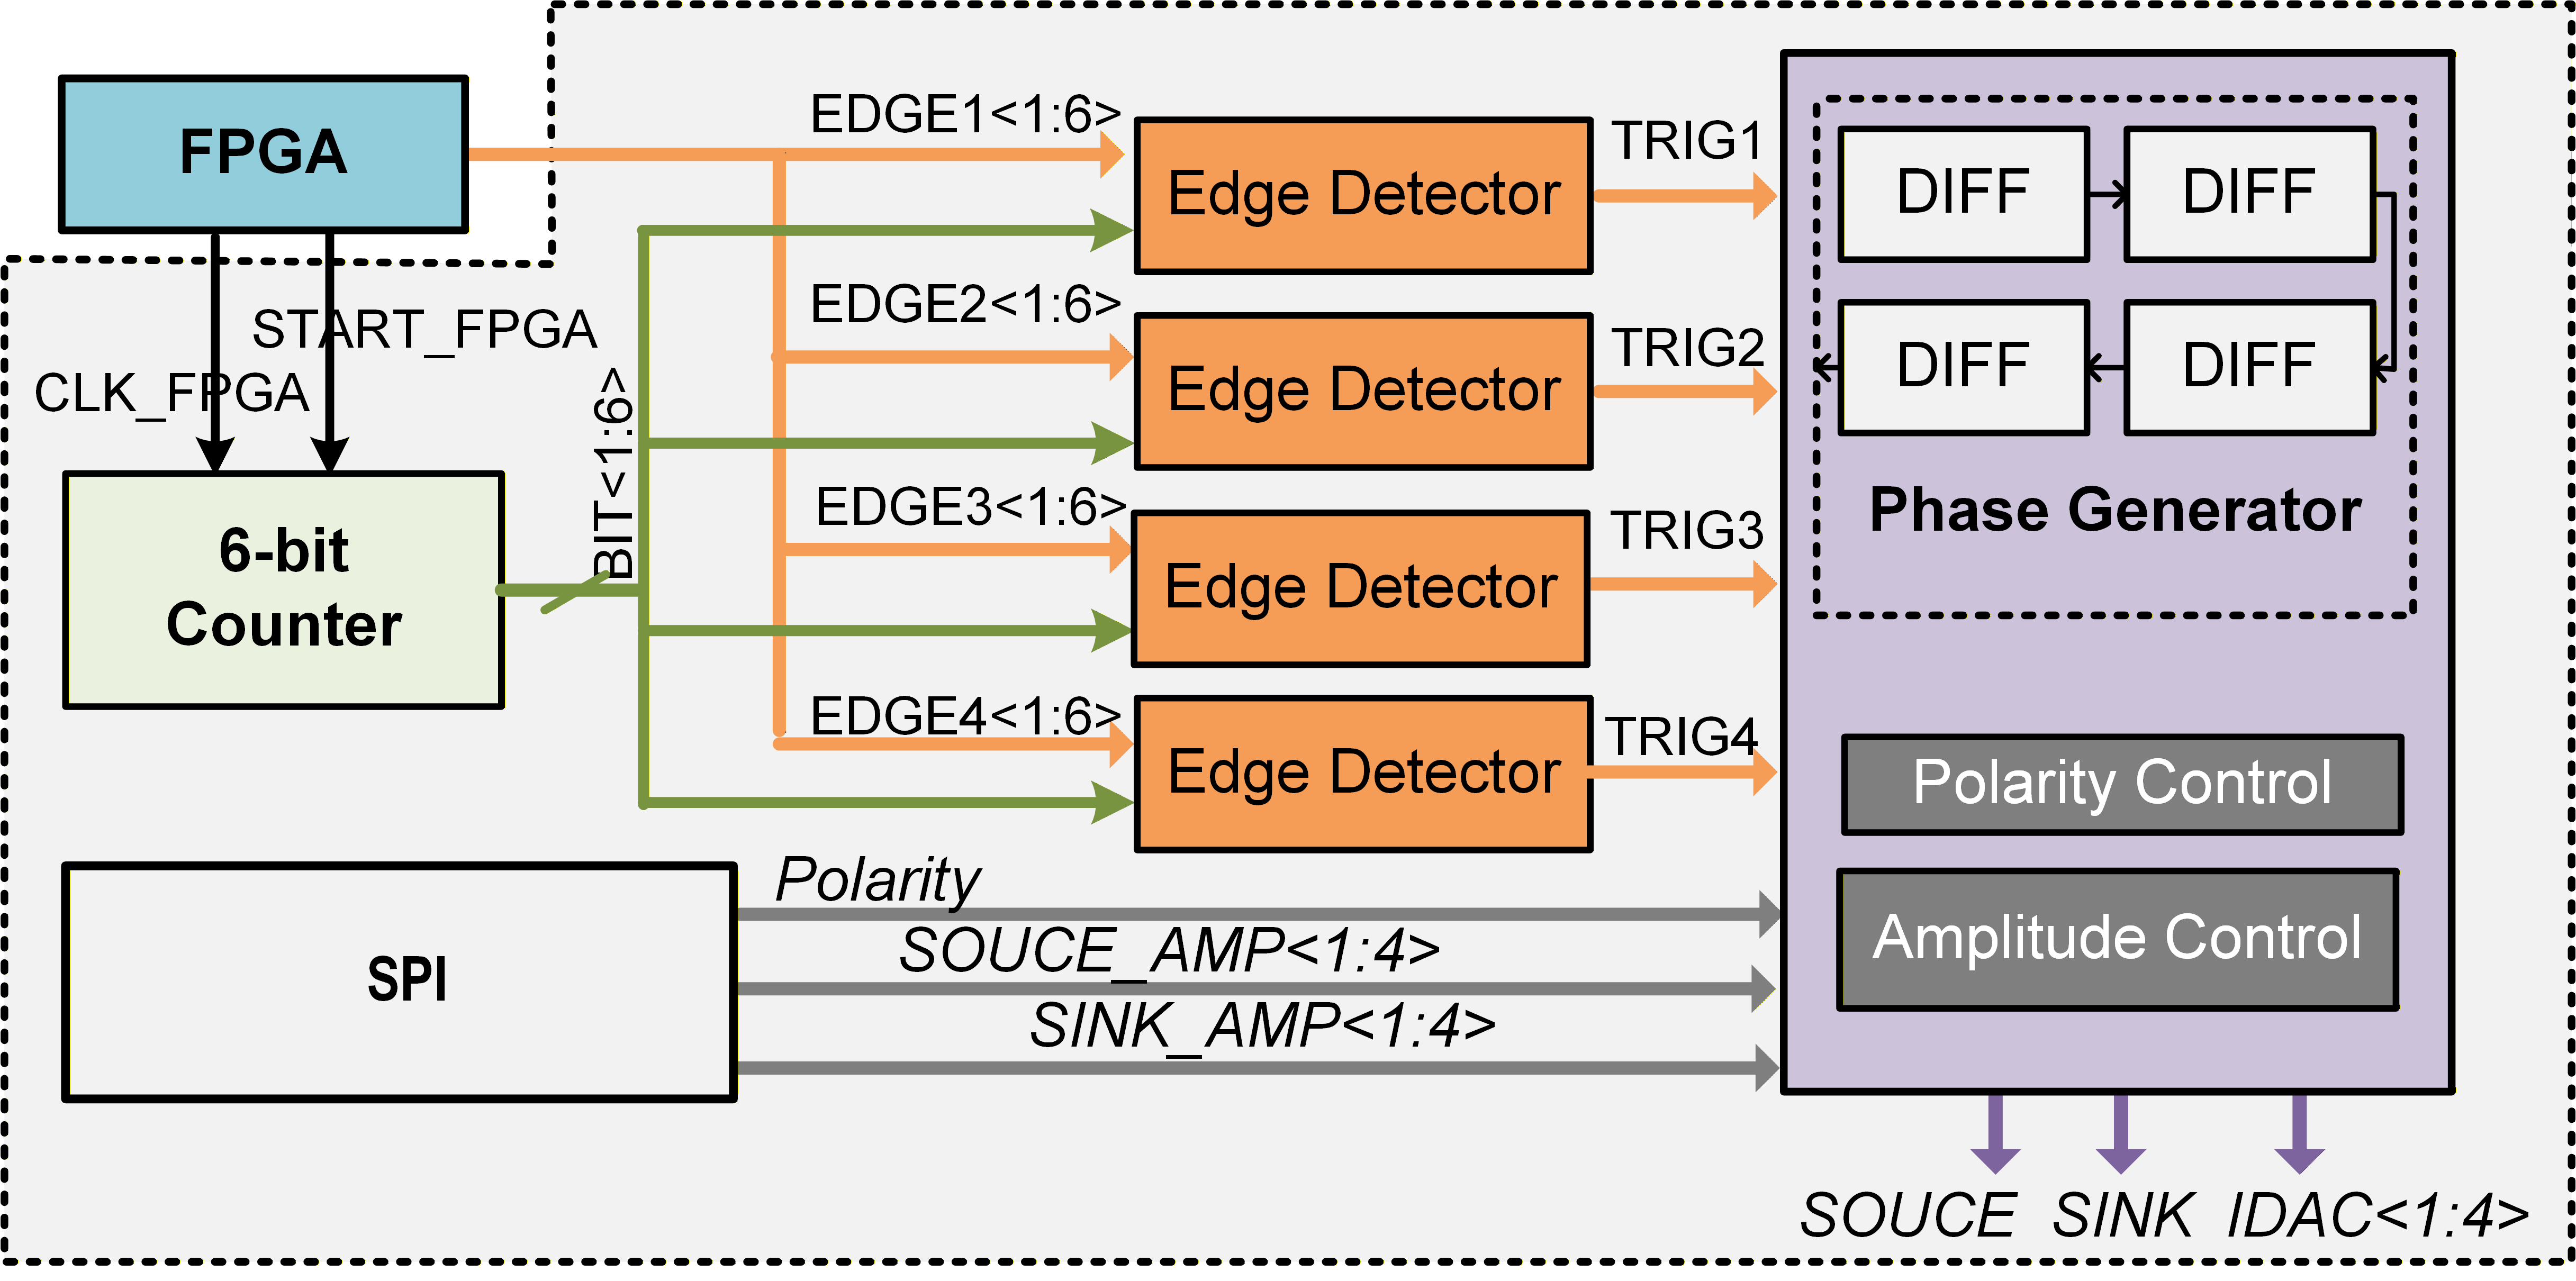
\includegraphics[width=3.5in]{3}
\caption{Programmable biphasic stimulation waveform generated by the proposed stimulator.}
\label{fig_3}
\end{figure}

The digital timing control circuitry generates the timing, polarity, and amplitude control signals required for biphasic stimulation. As shown in Fig.3, a 6-bit counter driven by \texttt{CLK\_FPGA} provides the global time reference $\mathrm{BIT}\langle1{:}6\rangle$. Programmable edge detector blocks compare $\mathrm{BIT}\langle1{:}6\rangle$ with the stored edge parameters $\mathrm{EDGE1}\langle1{:}6\rangle$ to $\mathrm{EDGE4}\langle1{:}6\rangle$, generating trigger events $\mathrm{TRIG1}$ to $\mathrm{TRIG4}$ at predefined timing points. These trigger signals are processed by sequential digital logic to produce phase signals $P_1$–$P_4$, which define the boundaries of the stimulation phases.

\begin{figure}[!t]
\centering
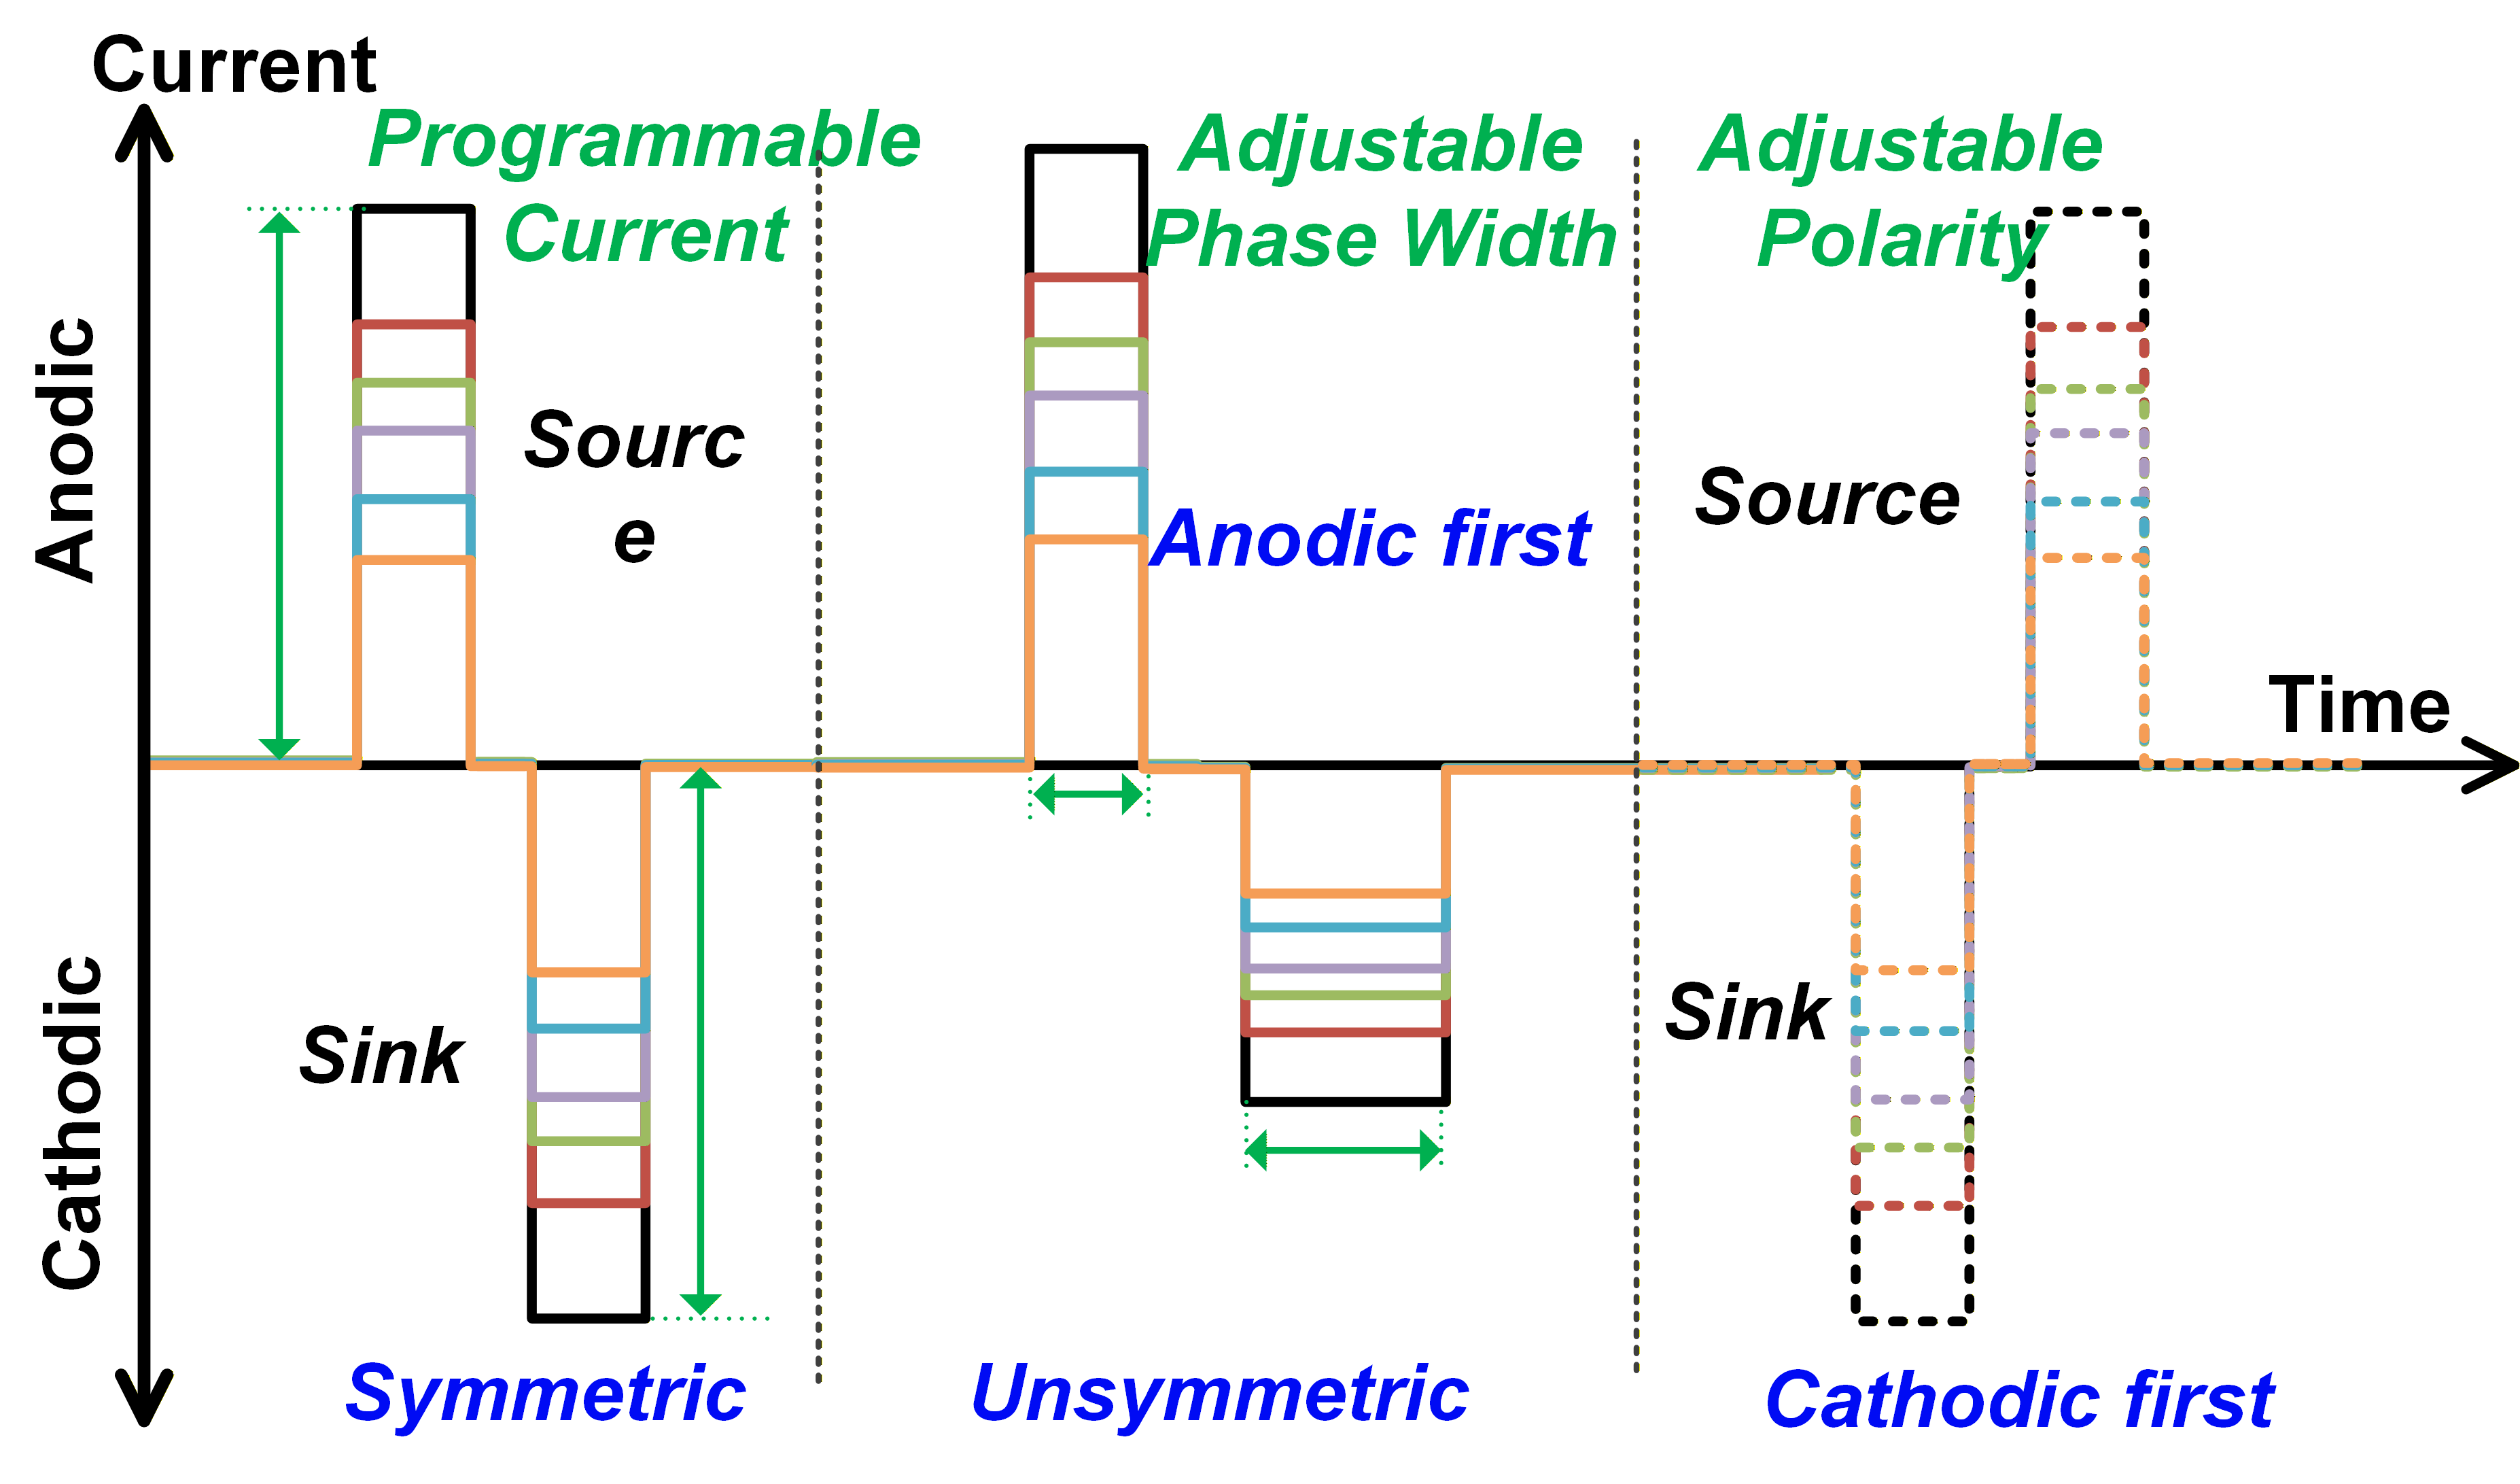
\includegraphics[width=3.2in]{4}
\caption{Programmable biphasic stimulation waveform generated by the proposed stimulator.}
\label{fig_4}
\end{figure}

Based on the generated phase signals and the programmed \texttt{POLARITY}, combinational logic activates either the \texttt{SOURCE} or \texttt{SINK} current path to produce biphasic stimulation. The stimulation amplitude is configured by the digital codes $\mathrm{SOURCE\_AMP}\langle1{:}4\rangle$ and $\mathrm{SINK\_AMP}\langle1{:}4\rangle$, which control a 4-bit current-steering DAC ($\mathrm{IDAC}\langle1{:}4\rangle$) that sets the stimulation current level.
Through this digital control architecture, the stimulator supports programmable pulse timing, polarity, inter-phase delay, and independently adjustable source/sink current amplitudes. Fig.~4 illustrates the programmable biphasic stimulation waveforms.

The programmable stimulation parameters are configured through a Serial Peripheral Interface (SPI). Each stimulator channel is controlled by a 33-bit configuration word that defines key stimulation parameters, including current amplitude, phase timing, and polarity. In this design, a single SPI controller configures four stimulator channels simultaneously, resulting in a total 132-bit control word. The received serial data are first shifted into a set of shift registers synchronized with \texttt{SCLK}. When the complete control word is received, the \texttt{LATCH} signal transfers the data into configuration registers, where the parameters are stored and distributed to the corresponding digital timing and stimulation control blocks. Through this SPI-based configuration scheme, stimulation parameters can be digitally programmed and updated across the stimulator array while maintaining deterministic timing and reliable operation.

\subsection{Power Supply Generation and Distribution}

The stimulator system requires multiple supply domains to support both the low-voltage digital control circuitry and the high-voltage stimulation output stage. The digital blocks developed in the previous sections, including the SPI interface and the digital timing control logic, operate in the low-voltage domain and are powered by an on-chip LDO that generates a 1.6~V supply. The stimulation output stage requires higher voltage compliance to drive neural electrodes and is therefore powered by external $\pm$10~V supplies.

Based on this supply partitioning, a power distribution scheme is established to separate the low-voltage digital/control domain from the high-voltage stimulation domain. The on-chip LDO provides a regulated 1.6~V supply for the SPI logic, timing control circuitry, and other digital blocks, while the external $\pm$10~V rails directly power the stimulator output stage.

The layout-level power organization is designed to ensure reliable power delivery and proper isolation between the supply domains. Separate routing structures are used for the low-voltage digital supply and the high-voltage stimulation rails, and the power connections are integrated with the stimulator array and digital control blocks to support stable system operation.

\section{Results}

The proposed stimulator system was implemented in a 180~nm BCD process. The layout area of a single stimulator cell is $358\,\mu m \times 96\,\mu m$, including the high-voltage stimulation circuitry and the local digital timing control logic. The stimulator employs a shared bias current of 150\,nA. With the added switches to disable the stimulation paths in the off-state, the off-state power consumption is 243.7 \,\text{nW}. The SPI-based configuration block occupies an area of $350\,\mu m \times 205\,\mu m$ and is used to program four stimulator channels through a 132-bit control word. The following results evaluate the implementation according to the success metrics defined in the project goals. 
Fig.6 demonstrates the programmability of symmetric biphasic stimulation, including both the cathodic and the anodic phases. The maximum stimulation current reaches 22.5 µA, which satisfies the design specification. In addition, a discharge function is implemented to ensure safety by removing residual charge. Fig.7 also illustrates asymmetric stimulation with charge balancing, where the current amplitudes and pulse widths of the cathodic and anodic phases can be independently adjusted to maintain overall charge balance. Fig.8 shows the simulated waveforms of four stimulators in one channel configured through the SPI interface and local digital control. The stimulation timing and current waveforms follow the programmed control sequence, indicating that the SPI-controlled configuration and stimulation timing operate as expected. This verifies the correct functionality of the stimulation control logic and timing generation.


\begin{figure}[!t]
\centering
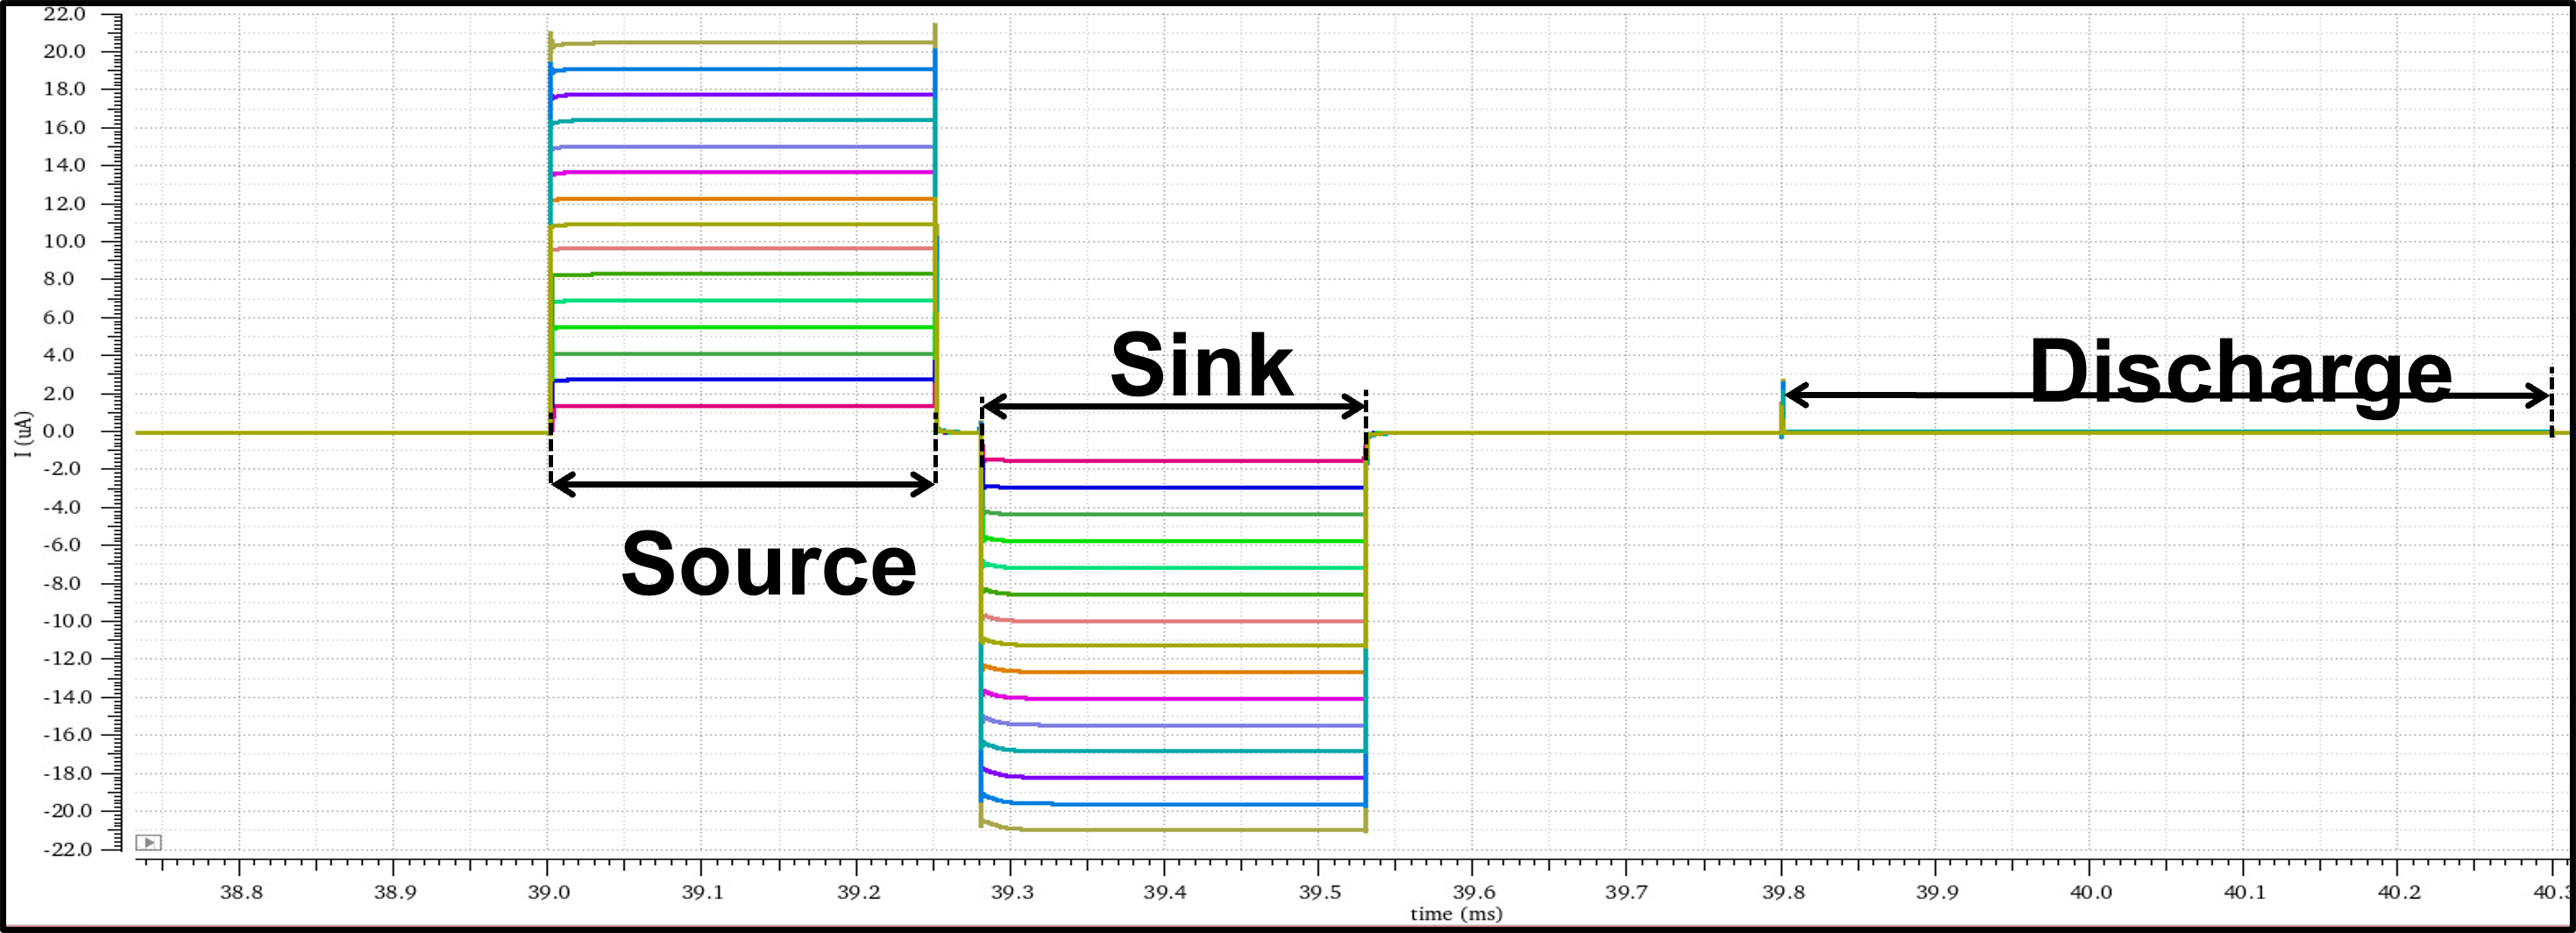
\includegraphics[width=3in]{r1.png}
\caption{The symmetric biphasic stimulation waveforms.}
\label{r1}
\end{figure}

\begin{figure}[!t]
\centering
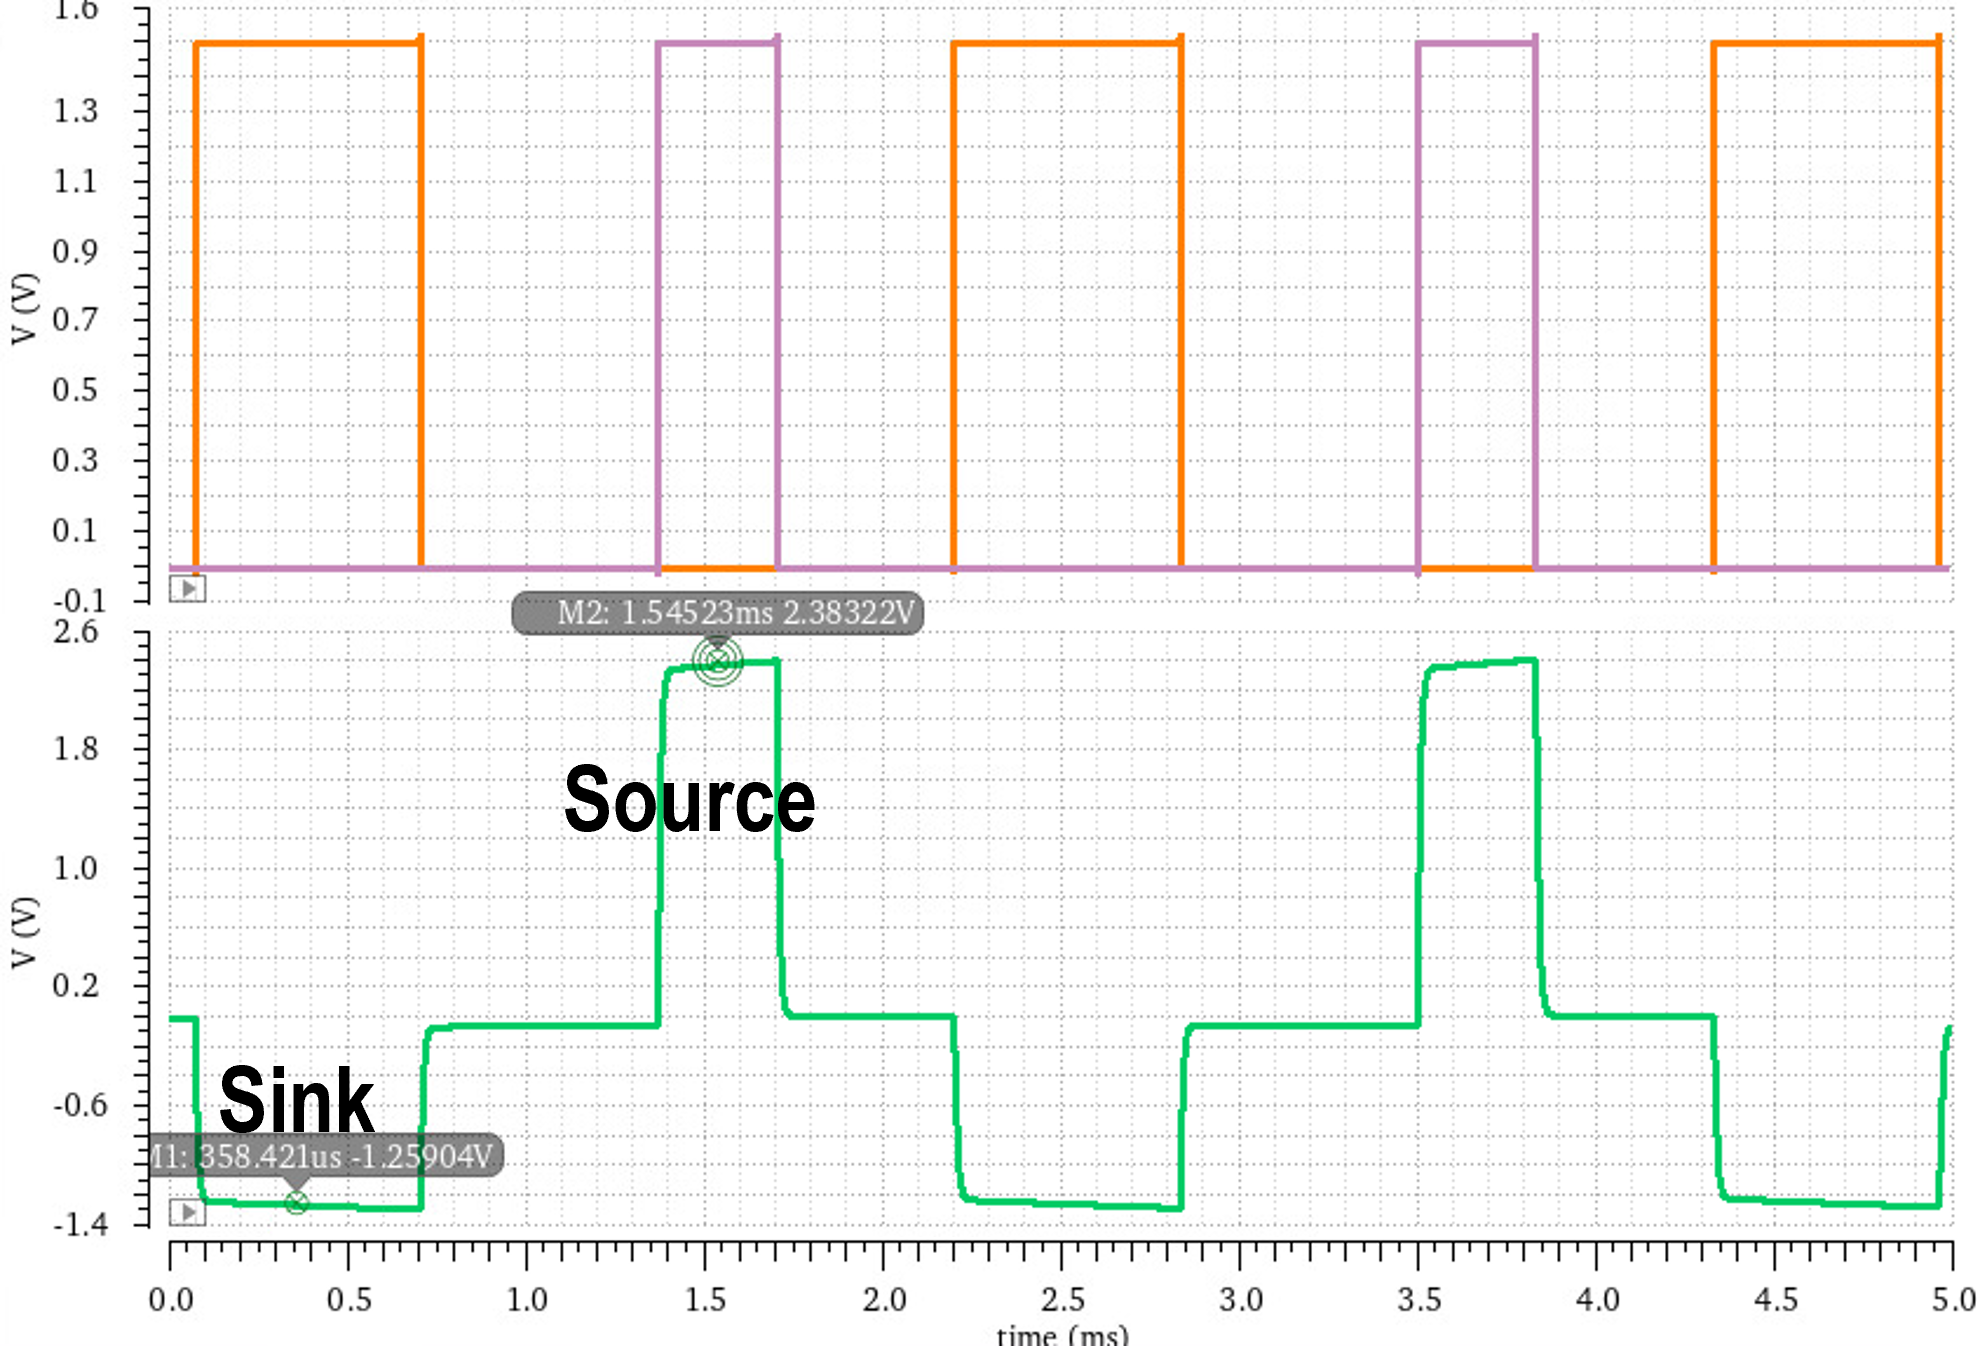
\includegraphics[width=3in]{r2.png}
\caption{The asymmetric biphasic stimulation waveforms.}
\label{r2}
\end{figure}

\begin{figure}[!t]
\centering
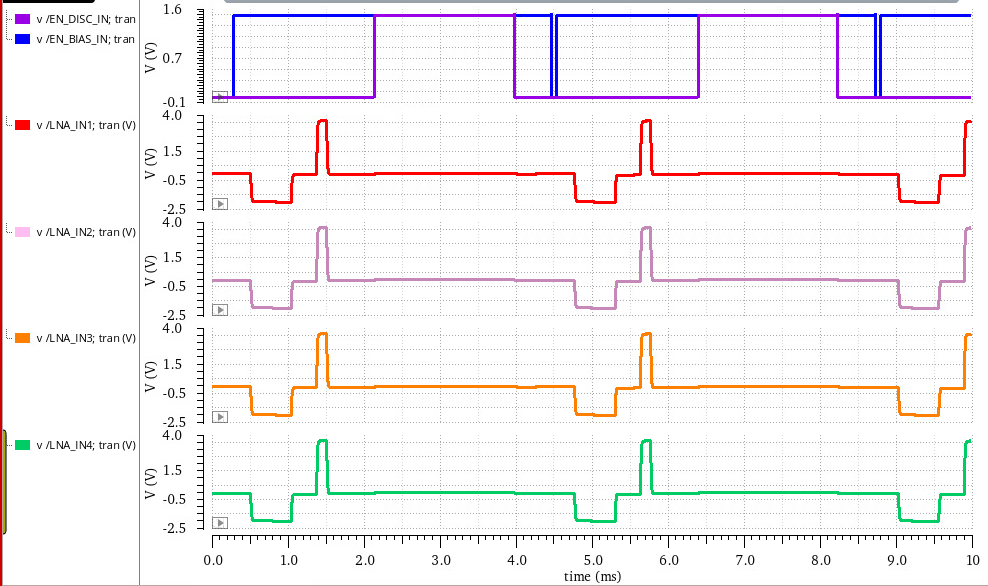
\includegraphics[width=3in]{r3.png}
\caption{Simulated waveforms of four stimulators in one channel controlled through the SPI interface.}
\label{r3}
\end{figure}

\section{Discussion}
The simulation results verify the correct operation of the proposed stimulator architecture and SPI-based configuration scheme. Programmable stimulation parameters enable flexible generation of symmetric and asymmetric charge-balanced biphasic waveforms. The maximum stimulation current reaches 22.5~µA, meeting the design target. The integrated discharge path ensures safe operation by removing residual charge after stimulation. In addition, the correct timing of multiple stimulators within a channel demonstrates the effectiveness and scalability of the digital control architecture.

Although the current implementation relies on wired power supplies, the proposed architecture provides a suitable foundation for future fully implantable systems. Future work will focus on developing a wireless power and data transfer (WPDT) system~\cite{ref13} to replace the present wired power supply structure. In the current design, the digital control circuitry is powered by an on-chip 1.6~V LDO, while the stimulator output stage is powered by external $\pm10$~V supplies.

To enable wireless operation, future work will investigate inductive wireless power delivery capable of generating these required supply domains. The WPDT system will employ an inductive link to transfer power and use on-chip rectification and regulation circuits to generate the necessary DC voltages. The rectifier topology, power conversion efficiency, and voltage generation capability will be optimized to support both the low-voltage digital control circuits and the high-voltage stimulation stage.


\section{Acknowledgments}
The author gratefully acknowledges support from the RISE research group for their valuable collaboration and input.
\section{CRediT Author Statement}
Conceptualization: Gerald Topalli, Yiling Xie. Methodology: Yiling Xie, Gerald Topalli. Circuit Design: Yiling Xie. Simulation and Validation: Yiling Xie  
Writing – original draft, review and editing: Yiling Xie  

\begin{thebibliography}{1}
\bibliographystyle{IEEEtran}

\bibitem{ref1}
J. Lee, V. Leung, A. H. Lee, N. B. Liu, and M. M. Maharbiz, ``Neural recording and stimulation using wireless networks of microimplants,'' \textit{Nature Electronics}, vol. 4, pp. 604--614, 2021.

\bibitem{ref2}
T. Jung, N. Zeng, J. D. Fabbri, R. W. Rios, and M. M. Maharbiz, ``A wireless subdural-contained brain--computer interface with 65,536 electrodes and 1,024 channels,'' \textit{Nature Electronics}, vol. 8, pp. 1272--1288, 2025.

\bibitem{ref3}
A. H. Lee, J. Lee, V. Leung, N. B. Liu, and M. M. Maharbiz, ``Patterned electrical brain stimulation by a wireless network of implantable microdevices,'' \textit{Nature Communications}, vol. 15, Art. no. 10093, 2024.

\bibitem{ref4}
S. A. M. Al Abed, C. B. Jeong, J. Lee, and H. J. Yoo, ``Monopolar biphasic stimulator with discharge function and negative level shifter for neuromodulation SoC integration in low-voltage CMOS process,'' \textit{IEEE Transactions on Biomedical Circuits and Systems}, vol. 15, no. 6, pp. 1320--1332, Dec. 2021.

\bibitem{ref14}
J. Kim, S. Park, H. Kim, H. Shin, and M. Je, ``A scalable 256-channel 12-mA 0.06\%-current-mismatch 22-V neurostimulator with real-time current calibration and compliance monitoring,'' \textit{IEEE J. Solid-State Circuits}, vol. 56, no. 8, pp. 2472--2484, Aug. 2021.

\bibitem{ref13}
T. Lu and S. Du, ``A three-phase regulating resonant-current-mode rectifier with bypass-capacitor residual-free charging for wireless power transfer,'' \textit{IEEE J. Solid-State Circuits}, 2025, doi: 10.1109/JSSC.2025.3597069.



\end{thebibliography}


\newpage

\vfill

\end{document}


